The principal source for Quasi-Monte-Carlo methods is the book by
Niederreiter~\cite{niederreiter}, which however is highly mathematical
in tone. This section should also serve as an informal introduction
to Niederreiter's book.

In $1$-D, it is easy to show that the discrepancy (the error made in calculating
the size of an object based on the sampling)
is at least $\epsilon_N \propto 1/N$  when the sample points~${\mathbf x}_l$ are uniformly distributed. 
The key fact is that there exist sets of points (`low discrepancy sequences')
for which
the  discrepancy does not increase very much as the number of dimensions increases.

The simplest of these sets to describe is that due to Halton. In $1$-D, it is
identical to a van der Corput sequence, which involves generating
numbers on the unit interval, using the reversed bit patterns of the positive integers.
It is best illustrated by example. Thus $2$~has the binary representation~$10$, so
the $2$nd element in the van der Corput sequence is $.01_2$ or $1/4$, $3=11_2$ so
the $3$rd element in the van der Corput sequence is $.11_2$ or $3/4$, $4=100_2$ so
the $4$th element in the van der Corput sequence is $.001_2$ or $1/8$. Hence the
first $7$ elements of the van der Corput sequence are (in eighths)
\begin{equation}
4,2,6,1,5,3,7
\end{equation}
It will be seen that there is a kind of fractal pattern about the above distribution.
Van der Corput  sequences may be defined for any prime~$b$, by representing the integers
in the base~$b$, then using the reversed representation as above to generate
values on the unit interval. The Halton sequence in $2$-D contains pairs
of numbers, the first in the $l$th pair being the $l$th element from a van der Corput sequence with base~$2$
and  the second being the corresponding element in a base~$3$ van der Corput sequence.
In fact any two distinct primes could be used, and the generalisation to
many dimensions should be obvious.

The discrepancy of the Halton sequence in $2$-D is bounded by
a formula which may be approximated as
\begin{equation}
\epsilon_N = A_2 (\ln N)^2/N
\end{equation} 
where $A_2=0.66$. It will be seen that this is smaller than
the Monte-Carlo value of $\epsilon_N = 1/\sqrt{N}$ for $N > 1000$. It
is therefore also competitive with uniform sampling on a rectangular lattice of $N$
$2$-D points,
which in general gives an error proportional to
lattice spacing, ie.~$1/\sqrt{N}$.

The explanation for the superior performance of the Halton sequence 
is illustrated by comparison between \Fig{ranlux} and \Fig{halton}.
Both show $100$ $2$-D vectors on the unit square, in fact the
last hundred of a length~$2000$ vector sequences starting at zero.
In \Fig{ranlux}, the components of the random vectors are generated
using the {\tt ranlux} random number generator (luxury level of~$3$ where $4$
is the highest) supplied by F.~James~\cite{Ja96RANL}.
\Fig{halton} plots the $2$-D Halton sequence generated
with base-2 and base-3 van der Corput sequences, using
a modified version of software due to J.~Burkardt~\cite{burkardt}
based on ref~\cite{Fo86Imple}.  It will be seen that,
comparing the number of points which are close together,
the random vectors are much less uniformly distributed than
the Halton sequence.

\begin{figure}
\centerline{\rotatebox{270}{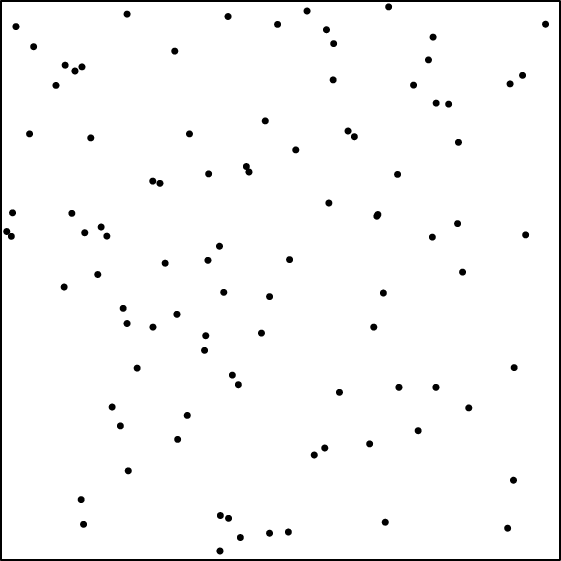
\includegraphics[width=6.5cm]{../png/ranlux1}}}
\caption{Two-dimensional vectors plotted by position in the unit square.
The {\tt ranlux} random number generator was used to produce $200$
coordinates, paired to make $100$~vectors.
\label{fig:ranlux}}
\end{figure}
\begin{figure}
\centerline{\rotatebox{270}{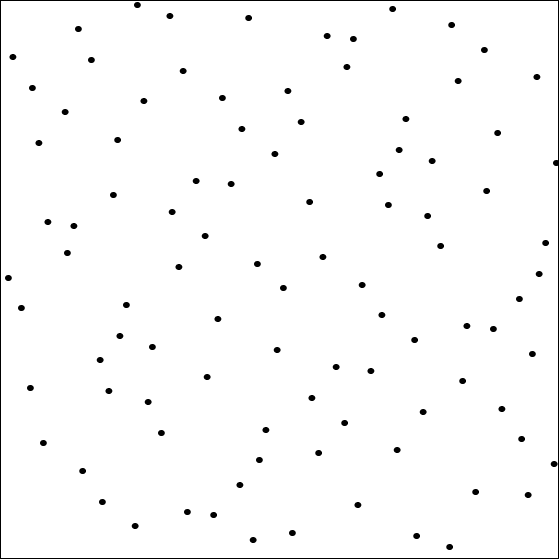
\includegraphics[width=6.5cm]{../png/halton1}}}
\caption{Two-dimensional vectors plotted by position in the unit square.
The {\tt halton} quasi-random number generator was used to produce $100$~vectors.
\label{fig:halton}}
\end{figure}

The Halton sequence is important because it can be defined without
setting a definite number of samples~$N_a$ in advance, hence it can be
used just like sequences from standard Monte-Carlo random number generators.
This contrasts with the Hammersley sequence, where the first component of
each vector is~$l/N_a$, then other components contain van der Corput sequences.
However, much of
Niederreiter's book is concerned with cases where $N_a$ is specified in advance,
when it transpires for example that $A_2$ may be reduced to as little as~$0.26$, using a $(t,s)$~sequence.

The definition of $(t,s)$~sequences is quite involved. The main idea is to
generate the quasi-random sequences as sets of vectors of dimension~$s$ 
(hence the $s$ in the name) rather than as in Halton where the components
of the vectors are computed independently as $1$-D van der Corput sequences.
The $t$ denotes the fact that, instead of each integer being represented in base~$b$
prior to bit reversal, it is represented in base~$b^{t+1}$. Hence,
in the $(t,s)$~notation,  van
der Corput sequences are $(0,1)$~sequences, and anyway apparently $t=0$
has optimally small error.
%Software for $(t,s)$~sequences
%is available from ACM~TOMS on the web~\cite{Br94Prog} and has been downloaded and tested.

Returning to Halton sequences,
the expression for discrepancy in $d$-D is
\begin{equation}
\epsilon_N = A_d (\ln N)^d/N
\end{equation} 
where the values of $A_d$ are tabulated in Niederreiter's Table~4.4.~\cite[p.96]{niederreiter}.
The first few are $A_d = 0.66, 0.82, 1.26, 2.62$, for~$d=2,3,4,5$. At higher~$d$,
$A_d$ increases rapidly so that for example, $A_{12} = 16\,800$ and
$A_{20}=6.62 \times 10^{10}$, whereas the corresponding value~$C_d$ for the
best $(t,s)$ sequence \emph{decreases} almost as rapidly ($C_6=0.0186$).
This is the benefit  gained from the greater complexity of 
calculating the $(t,s)$~sequences.

Despite the theory, much practical experience with QMC
as reported and performed by Morokoff~\emph{et al}~\cite{Mo94Quas,Mo95Quas}
suggests that QMC frequently performs little better than MC
when $d$ is large. Morokoff~\emph{et al} considered Halton sequences
and $(t,s)$ sequences in base~$b=2$ (referred to as Sobol sequences)
and in other prime number bases (Faure sequences).
It seems that for the variety of methods tested,
the number of sample points required for the asymptotic discrepancy
estimates to be realised can increase exponentially with dimension~$d$,
so the curse of dimensionality remains.
There is evidence however that in some problems, where only a relatively small
number of dimensions is apparently important, QMC performance
can be greatly improved~\cite{Ca97Valu}. One important point to make
is that Morokoff~\emph{et al} tended to explore more those QMC
rules which had the best asymptotic behaviour. Their results do not
exclude the possibility that the simpler techniques of
lattice rules, see ref~\cite[\S\,5.1]{niederreiter},
might have better behaviour in
practice, especially if the lattice basis~${\mathbf g}$ is well chosen.
Note that NAG uses the simple Korobov rule, in which the components of~${\mathbf g}$
are given as
\begin{equation}
g_k = a^{(k-1)} (\mod p)
\end{equation}
 for specially chosen real~$a>1$ and prime number~$p$.
%if Q is discontinuous or K is large

